\section{Phần 1. Trực quan hóa và phân tích}

\subsection{Demand-side}
Từ phần tổng quan trong Synthesis, có thể thấy doanh nghiệp vẫn duy trì được tăng trưởng người đăng ký, nhưng số đơn hàng và doanh thu chưa tăng tương xứng, đồng thời dao động đáng kể theo thời gian. Điều này cho thấy \textbf{điểm nghẽn chính nằm ở demand-side}: khách đi vào hệ thống nhưng chưa được chuyển hóa ổn định thành hành vi mua lặp lại.

\begin{figure}[h]
  \centering
  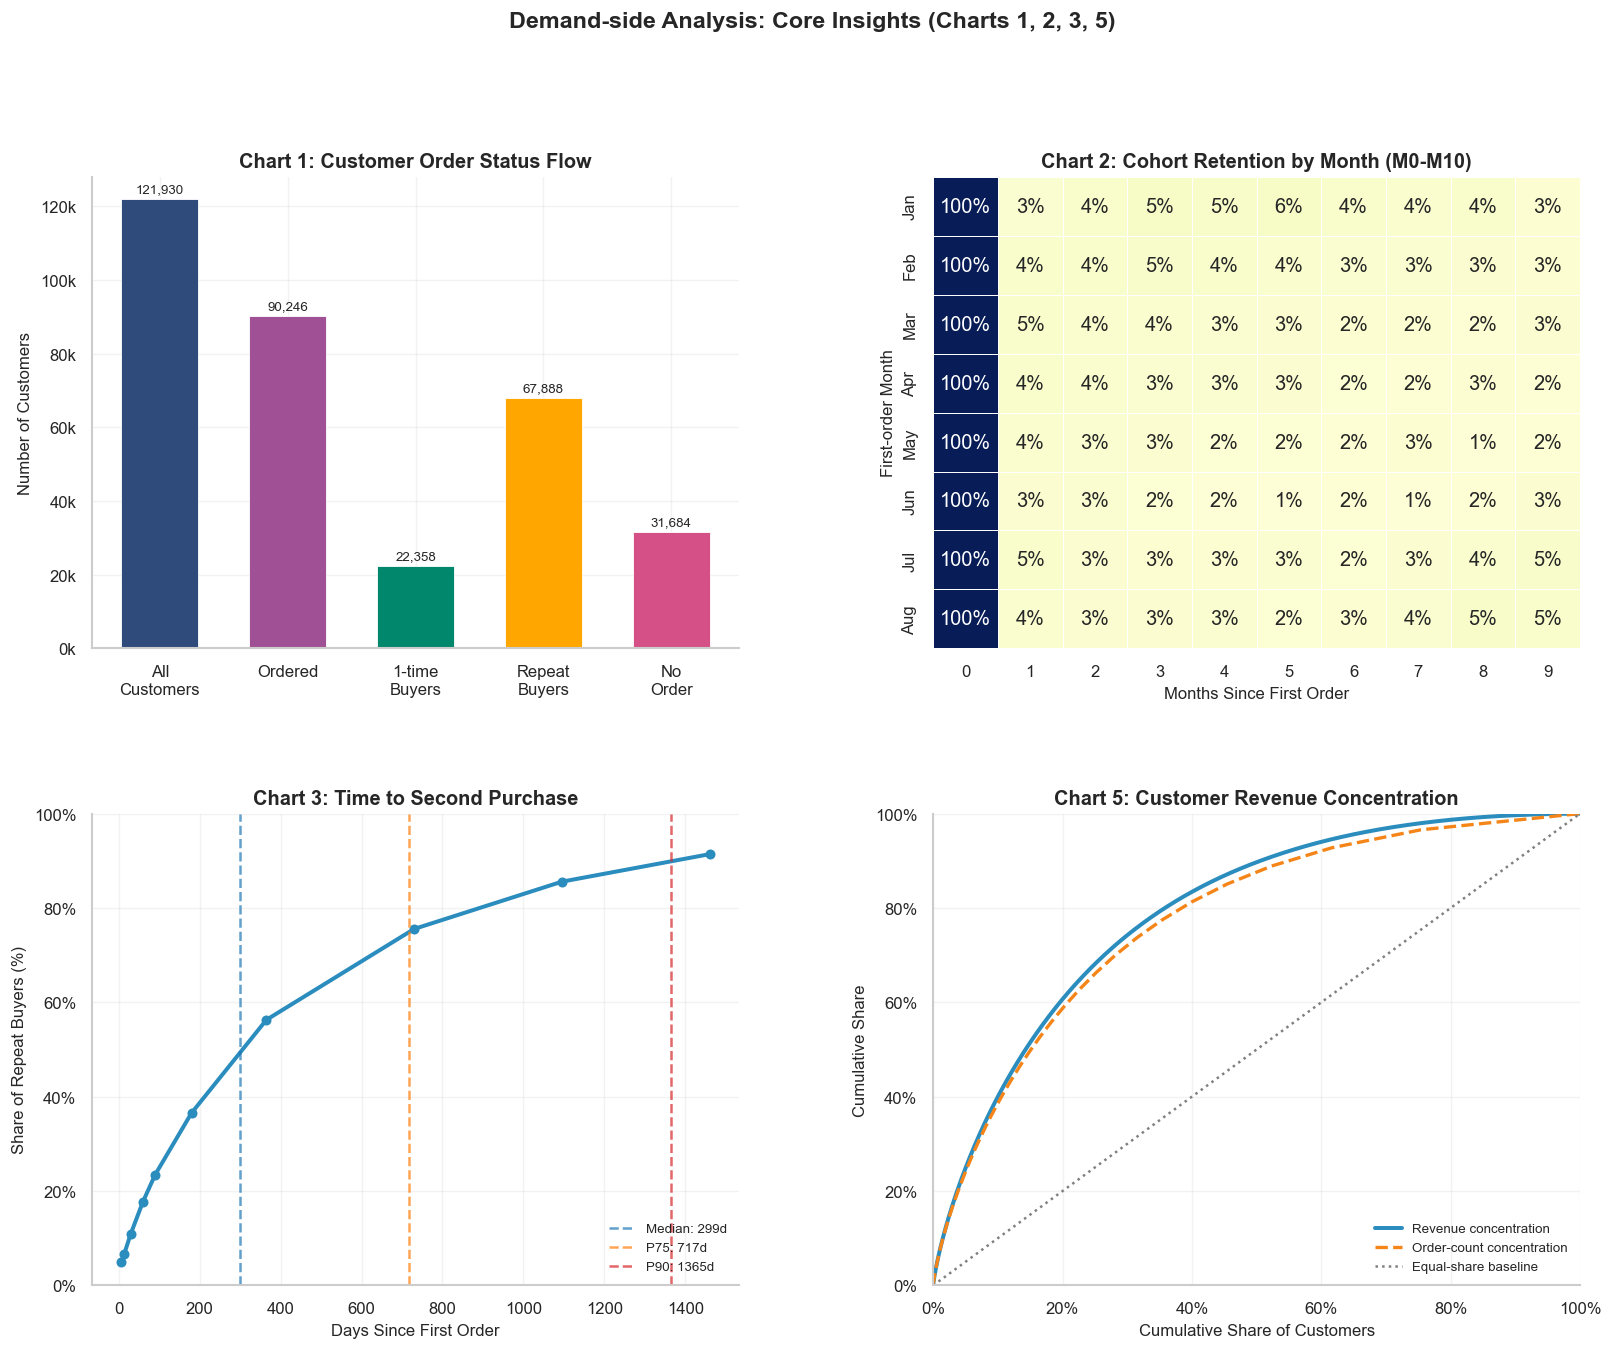
\includegraphics[width=0.98\linewidth]{demand.png}
  \caption{Demand-side Analysis: Core Insights (Charts 1, 2, 3, 5) tập hợp phễu chuyển đổi, retention theo cohort, thời gian mua lại, và phân bố doanh thu.}
  \label{fig:demand_composite}
\end{figure}

Phân tích phễu chuyển đổi cho thấy \textbf{rò rỉ xuất hiện ở hai lớp}: trước đơn hàng đầu tiên và ngay sau đơn hàng đầu tiên. Nghĩa là doanh nghiệp không chỉ mất khách ở bước acquisition, mà còn mất tiếp ở activation và giữ chân sớm. Khi đi sâu vào nhóm đã qua đơn đầu, retention cho thấy \textbf{nhịp quay lại không đồng đều theo cohort và theo mùa}, vì vậy không thể dùng một công thức chung cho mọi khách hàng. Nếu không quản trị theo cohort, doanh nghiệp rất dễ đánh giá sai chất lượng demand và phân bổ ngân sách CRM thiếu hiệu quả.

Kết quả về thời gian đến lần mua thứ hai tiếp tục củng cố rằng \textbf{khách quay lại muộn hơn kỳ vọng}, thay vì biến mất hoàn toàn. Do đó, việc chỉ đo trong khung 30--90 ngày có thể tạo kết luận sai về churn. Đồng thời, phân bố doanh thu cho thấy \textbf{giá trị tập trung vào một nhóm khách hàng nhỏ} và đi cùng tần suất mua, nên tăng trưởng bền vững cần quản trị theo tầng giá trị thay vì dàn đều nguồn lực cho toàn bộ tệp.

Trong 90 ngày tới, ưu tiên thực thi gồm ba trục: \textbf{(1) giảm rò rỉ đầu phễu} bằng cách tăng chuyển đổi từ signup sang first order; \textbf{(2) điều khiển retention theo cohort và theo cửa sổ dài hơn} để bắt đúng nhịp mua lại; \textbf{(3) tối ưu cơ cấu doanh thu} bằng cách tăng tỷ trọng nhóm Mid-high và giảm phụ thuộc vào tầng Top. Bộ KPI theo dõi hàng tuần gồm uplift chuyển đổi, tỷ lệ mua lại theo cohort, và mức độ tập trung doanh thu theo tầng khách hàng. Tổng hợp lại, nút thắt của demand-side không phải thiếu khách hàng theo nghĩa tuyệt đối, mà là mất khách theo từng chặng của hành trình và chậm nhịp repeat demand.

\subsection{Supply-side}
Phần 1.2 sẽ được nhóm phụ trách Supply-side bổ sung sau. Nội dung dự kiến tập trung vào năng lực đáp ứng nhu cầu theo danh mục/phân khúc, các điểm nghẽn stockout-overstock, và mức độ đồng bộ giữa tín hiệu demand với quyết định phân bổ tồn kho.

\section{Phần 2. Mô hình dữ liệu}
Phần này chưa triển khai trong phạm vi hiện tại và sẽ được hoàn thiện ở bước tiếp theo.